\documentclass[12pt, dvipdfmx]{beamer}

\renewcommand{\kanjifamilydefault}{\gtdefault}
%%%%%%%%%%%  package  %%%%%%%%%%%
\usepackage{bxdpx-beamer}% dvipdfmxなので必要
\usepackage{pxjahyper}% 日本語で'しおり'したい

\usepackage{amssymb,amsmath,ascmac}

\usepackage{multirow}
\usepackage{bm}

\graphicspath{{../../../Figures/gakkai/}}

\usepackage{tikz}
\usepackage{xparse}

\usepackage{multimedia}

\usetikzlibrary{shapes,arrows}
%% define fancy arrow. \tikzfancyarrow[<option>]{<text>}. ex: \tikzfancyarrow[fill=red!5]{hoge}
\tikzset{arrowstyle/.style n args={2}{inner ysep=0.1ex, inner xsep=0.5em, minimum height=2em, draw=#2, fill=black!20, font=\sffamily\bfseries, single arrow, single arrow head extend=0.4em, #1,}}
\NewDocumentCommand{\tikzfancyarrow}{O{fill=black!20} O{none}  m}{
\tikz[baseline=-0.5ex]\node [arrowstyle={#1}{#2}] {#3 \mathstrut};}

%微分関連のマクロ
%
\newcommand{\diff}{\mathrm d}
\newcommand{\difd}[2]{\dfrac{\diff #1}{\diff #2}}
\newcommand{\difp}[2]{\dfrac{\partial #1}{\partial #2}}
\newcommand{\difdd}[2]{\dfrac{\diff^2 #1}{\diff #2^2}}
\newcommand{\difpp}[2]{\dfrac{\partial^2 #1}{\partial #2^2}}

%目次スライド
\AtBeginSection[]{
  \frame{\tableofcontents[currentsection]}
}

%アペンディックスのページ番号除去
\newcommand{\backupbegin}{
   \newcounter{framenumberappendix}
   \setcounter{framenumberappendix}{\value{framenumber}}
}
\newcommand{\backupend}{
   \addtocounter{framenumberappendix}{-\value{framenumber}}
   \addtocounter{framenumber}{\value{framenumberappendix}} 
}

\newcommand{\rmd}{\mathrm{d}}
\newcommand{\dd}[1]{\dfrac{\mathrm{d} #1}{\mathrm{d} x}}

%%%%%%%%%%%  theme  %%%%%%%%%%%
\usetheme{Copenhagen}
% \usetheme{Metropolis}
% \usetheme{CambridgeUS}
% \usetheme{Berlin}

%%%%%%%%%%%  inner theme  %%%%%%%%%%%
% \useinnertheme{default}

% %%%%%%%%%%%  outer theme  %%%%%%%%%%%
\useoutertheme{default}
% \useoutertheme{infolines}

%%%%%%%%%%%  color theme  %%%%%%%%%%%
%\usecolortheme{structure}

%%%%%%%%%%%  font theme  %%%%%%%%%%%
\usefonttheme{professionalfonts}
%\usefonttheme{default}

%%%%%%%%%%%  degree of transparency  %%%%%%%%%%%
%\setbeamercovered{transparent=30}

% \setbeamertemplate{items}[default]

%%%%%%%%%%%  numbering  %%%%%%%%%%%
% \setbeamertemplate{numbered}
\setbeamertemplate{navigation symbols}{}
\setbeamertemplate{footline}[frame number]

%%%%%%%%%%%%%%%%%%%%%%%%%%%%%%%%%%%
\title
[ランダムな接続性を有するネットワークポリマーの緩和挙動]
{ランダムな接続性を有する\\ネットワークポリマーの緩和挙動}
\author[東亞合成 佐々木]{佐々木裕}
\institute[東亞合成]{東亞合成}
\date{October 21, 2021}
%%%%%%%%%%%%%%%%%%%%%%%%%%%%%%%%%%
\begin{document}
%%%%%%%%%%%%%%%%%%%%%%%%%%%%%%%%%%
\begin{frame}\frametitle{}
	\titlepage
\end{frame}
% %%%%%%%%%%%%%%%%%%%%%
% \section*{}
% %
% \begin{frame}
% %[allowframebreaks]
% {Outline}
% 	\tableofcontents
% \end{frame}

%%%%%%%%%%%%%%%%%%%%%
\section{はじめに}
%%%%%%%%%%%%%%%%%%%%%%%%%%%%%%%%%%%%%%%%%%%%%
\subsection{背景}

\begin{frame}
	\frametitle{高分子材料への期待と不安}
	地球温暖化対策の CO$_2$ 削減へ向けて、\\
	{\color{red}「自動車を中心とした運送機器の抜本的な軽量化」}
	\\
	が提唱されている。
	\begin{block}{高分子材料への期待}
		\begin{itemize}
			\item 現行の鉄鋼主体$ \Rightarrow$ 高分子材料を含むマルチマテリアル化
			\item 高分子材料によるマルチマテリアル化のポイント
				\begin{itemize}
					\item 高い比強度の有効利用
					\item 特徴を生かした適材適所 $\Leftrightarrow$ 適切な接合方法の選択
						\begin{itemize}
							\item {\color{red} 「接着接合」への高分子の利用}
							\item {\color{red} 「柔らかさを生かした弾性接着接合」}
							\item 耐久性、可逆性に優れた材料としてゴム材料に注目
						\end{itemize}
					\item {\color{blue}耐久性が不明確(特に疲労破壊に対して)}
				\end{itemize}
		\end{itemize}
	\end{block}
\end{frame}

% \begin{frame}
%     \frametitle{本研究の目標とアプローチ}
%         \begin{block}{目標}
%                 \begin{itemize}
%                     \item 高分子材料の破壊耐性向上の設計指針を得たい。
%                     \item 耐久性、可逆性に優れた材料としてゴム材料を選択
%                 \end{itemize}
%         \end{block}
% 		\begin{exampleblock}{アプローチ}
%             \begin{itemize}
%                 \item 実験的アプローチ
%                 \begin{itemize}
%                     \item 構造明確な\alert{三分岐}ネットワークを超分子で構築
%                     \item フィラー無添加での\alert{高い破断伸びと強度}
%                     \item 既知のモデルとの多数の整合点と、\alert{よくわからない点}。
%                 \end{itemize}
%                 \item マルチスケールシミュレーションで\color{red}モデル\color{black}を構築
%                 \begin{itemize}
%                     \item 単純化したモデルで小さなスケールから始めたい。
%                     \item \alert{長さの揃ったストランドで MD シミュレーション}
%                     % \item 最終的に、亀裂先端の挙動を FEM シミュレーション
%                 \end{itemize}
%             \end{itemize}
% 		\end{exampleblock}
% \end{frame}

\subsection{ゴム材料の破壊}
\begin{frame}
    \frametitle{破壊工学の考え方}
    \begin{exampleblock}{破壊工学の考え方}
    
    \begin{itemize}
    \item
    系中に\alert{クラックが存在することを前提}に耐久性を評価
    % \item
    % \alert{「クラック近傍での応力集中を如何に抑制するか?」}
    \end{itemize}
    \end{exampleblock}
    \begin{columns}[totalwidth=1\textwidth]
    \column{.52\textwidth}
    \begin{alertblock}{破壊工学の観点から(微視的)}
        \begin{itemize}
            \item
            クラック先端の応力集中\\ \alert{応力拡大係数 $K_I$ で評価}
            \footnotesize
            \begin{align*}
            K_{I} = \sigma \sqrt{\pi c}
            \end{align*}
            \normalsize
            \item 
            クラック進展の抑制 \\
            $\Rightarrow$ 先端での\alert{局所降伏}\\
            降伏応力 $\sigma_Y$ に反比例
            \footnotesize
            \begin{align*}
            d \propto \left( \dfrac{K_I}{\sigma_Y} \right)^2
            \end{align*}
            \normalsize
        \end{itemize}
    \end{alertblock}
    \column{.46\textwidth}
        \centering
        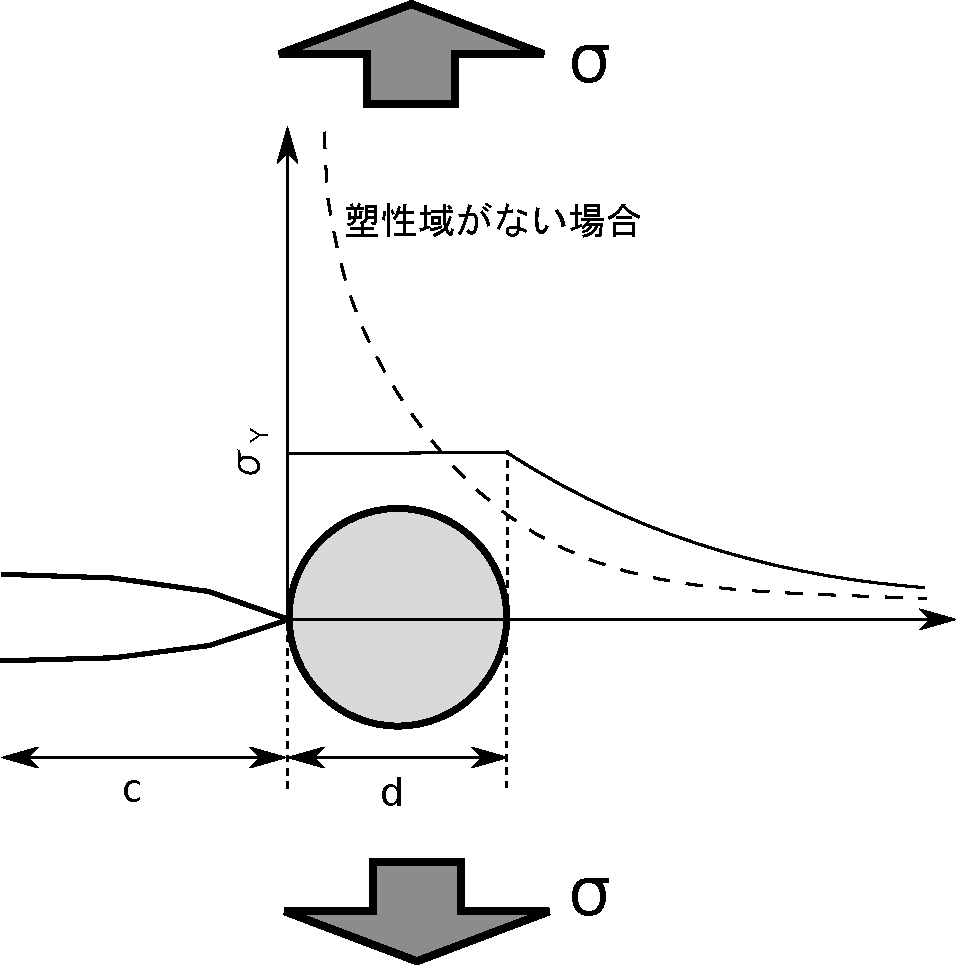
\includegraphics[width=0.9\textwidth]{./Crack_Yield.pdf}
    \end{columns}
\end{frame}

\begin{frame}
	\frametitle{ゴムの破壊と粘弾性}
		\begin{alertblock}{ゴムの破壊}
			大変形を伴う非線形現象だが、\\時間温度換算則の成立が多数報告
		\end{alertblock}
		\vspace{2mm}
		\begin{columns}[T, totalwidth=\textwidth]
			\column{.48\textwidth}
				亀裂先端近傍での大変形
				\vspace{-3mm}
				\begin{center}
					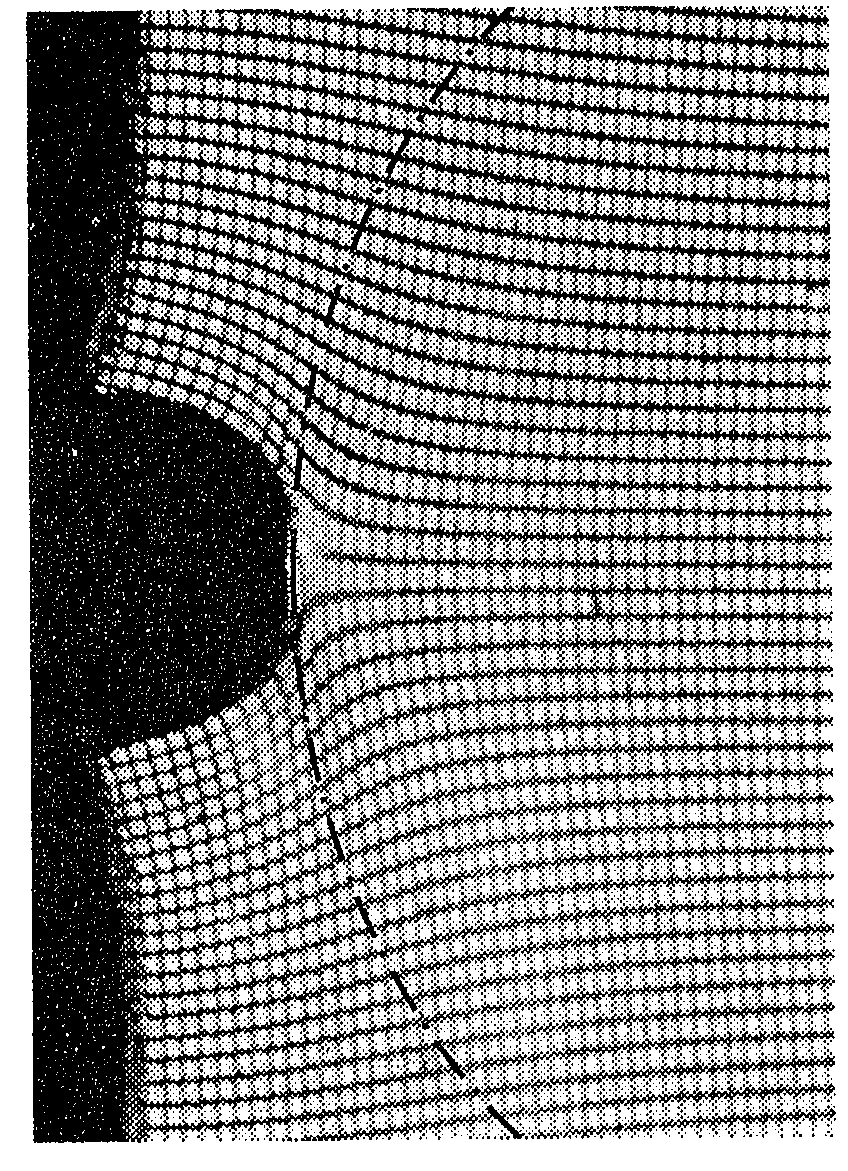
\includegraphics[width=.6\textwidth]{rubber_crack.png}
				\end{center}
			\column{.48\textwidth}
				時間温度換算則の成立
				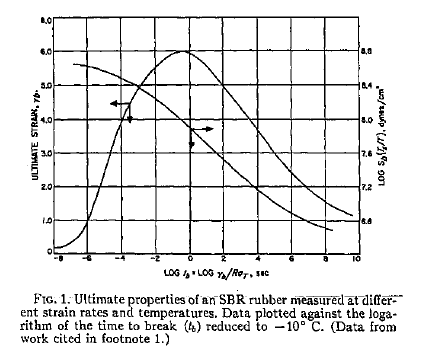
\includegraphics[width=.8\textwidth]{Time_Temp_2.png}

				{\tiny Smith T., Stedry P., J. Appl. Phys. (1960) 31 1892}
		\end{columns}
\end{frame}

\begin{frame}
    %[shrink squeeze]
    \frametitle{ゴムの破断強度の時間温度依存}
    
    %\begin{alertblock}{時間温度換算則で考えてみれば?}
    %NR の適正な変形速度・温度と SBR のそれとの違い
    %\end{alertblock}
    %
    
    \begin{columns}[T, totalwidth=\textwidth]
    \column{.53\textwidth}
    \begin{itemize}
		\item 粘弾性極限において\\
		(高温・低速)
	\end{itemize}
    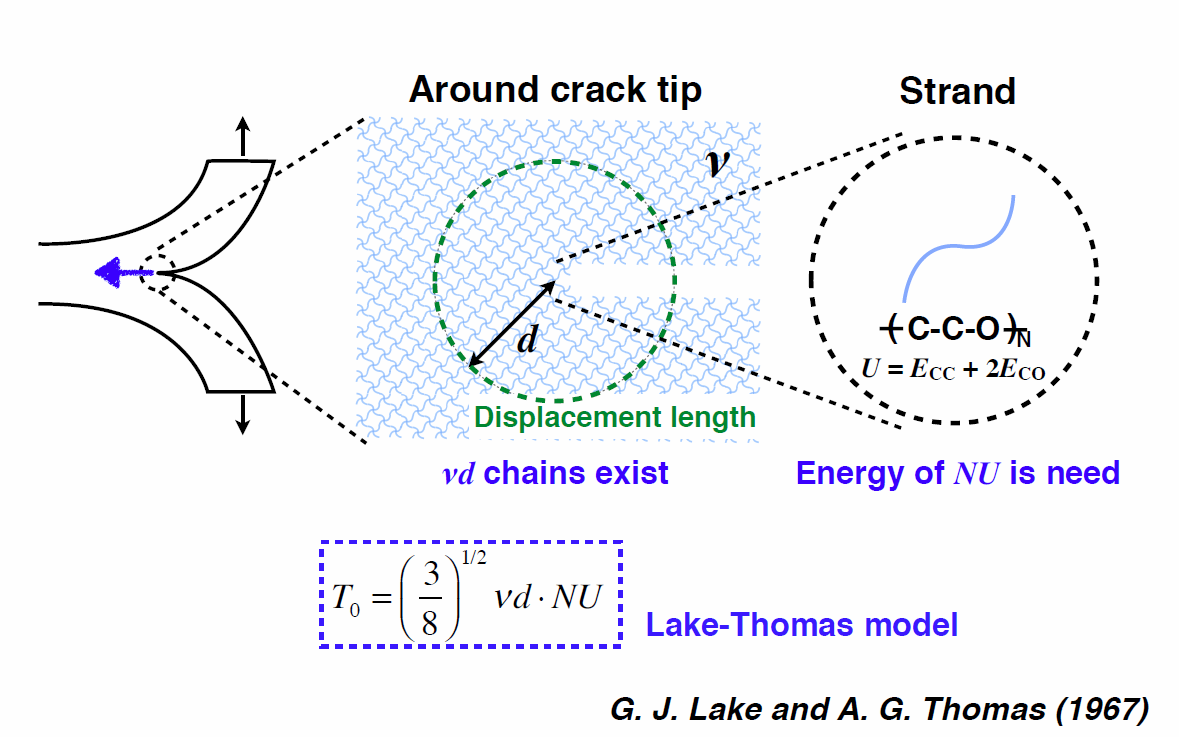
\includegraphics[width=\textwidth]{Lake_Thomas.png}
    
    \column{.45\textwidth}
    \begin{itemize}
		\item 変形速度、温度に依存\\
		破壊包絡線
	\end{itemize}
	\begin{center}
		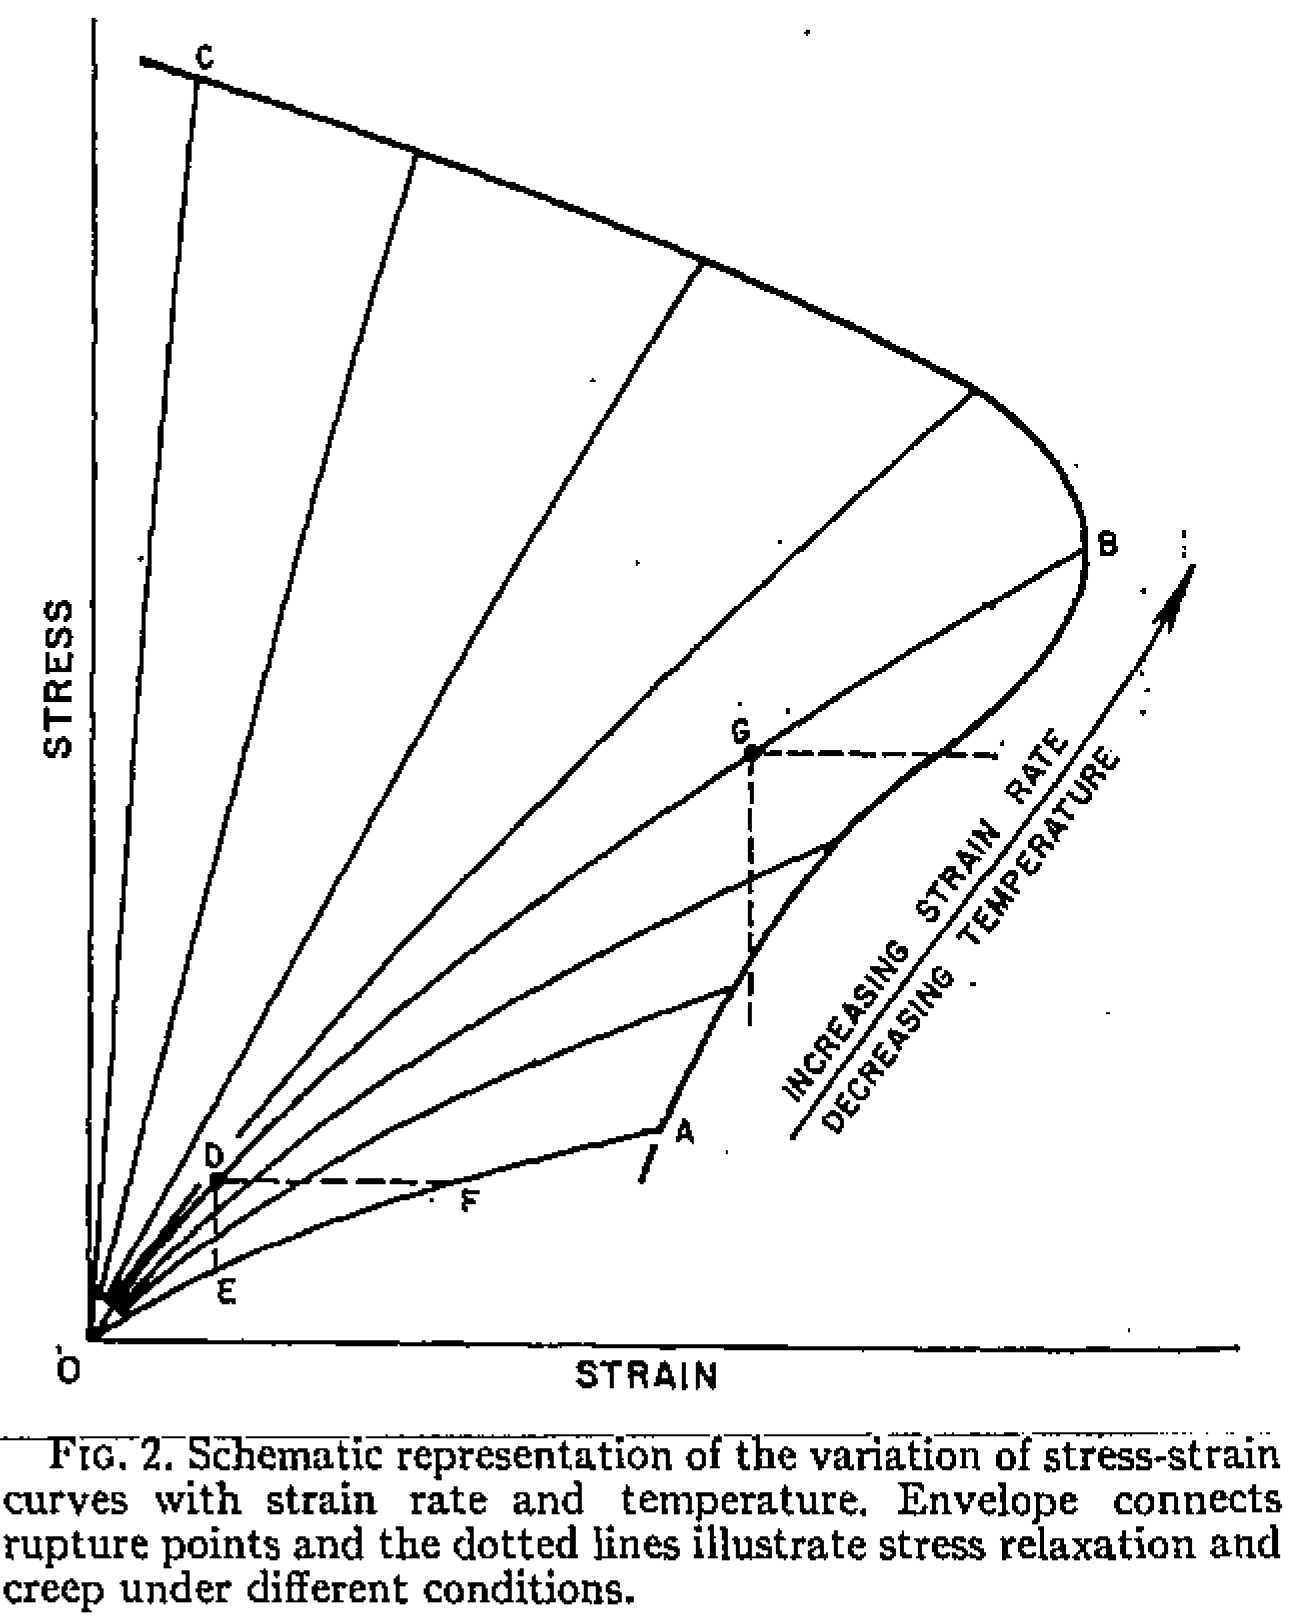
\includegraphics[width=.48\textwidth]{Time_Temp_3.png}

		{\tiny Smith T., Stedry P., J. Appl. Phys. (1960) 31 1892}
	\end{center}
    \end{columns}
    \begin{alertblock}{ゴムの引き裂きエネルギー}
		\vspace{-5mm}
		\begin{align*}
			&\mathcal{T}=\mathcal{T}_0 \Phi(\dot{c}, T, \epsilon_0) \\
			&\text{where $\dot{c}$ is crack velocity and $\epsilon_0$ is applied strain}
		\end{align*}
    % $\mathcal{T}=\mathcal{T}_0 \Phi(\dot{c}, T, \epsilon_0)$
    \end{alertblock}
\end{frame}

\begin{frame}
	\frametitle{Andrews 理論}
	\begin{columns}[totalwidth=1\textwidth]
		\column{.65\textwidth}
		\begin{exampleblock}{Andrews 理論}
		%クラック成長時の応力場の考察より
			\begin{itemize}
			\item
			降伏、ヒステリシスを示す材料
				\begin{itemize}
				\item
				\textcolor{blue}{Loading 場とUnloading 場}
				\item
				\alert{この差}が、全体の変形に要したエネルギーの多くを\alert{散逸}
				\item
			鎖の破断へのエネルギーが低減 \\$\Rightarrow$ \alert{強靭さの起源。}
				\end{itemize}	
			\item
			\textcolor{green}{実験的に、$\Phi$ を求めている。}
			\end{itemize}
		\end{exampleblock}
		
		{Andrews, E. H. and Fukahori, Y., J. of Mat. Sci., 12, 1307 (1977)}
		
		\column{.35\textwidth}
		\centering
		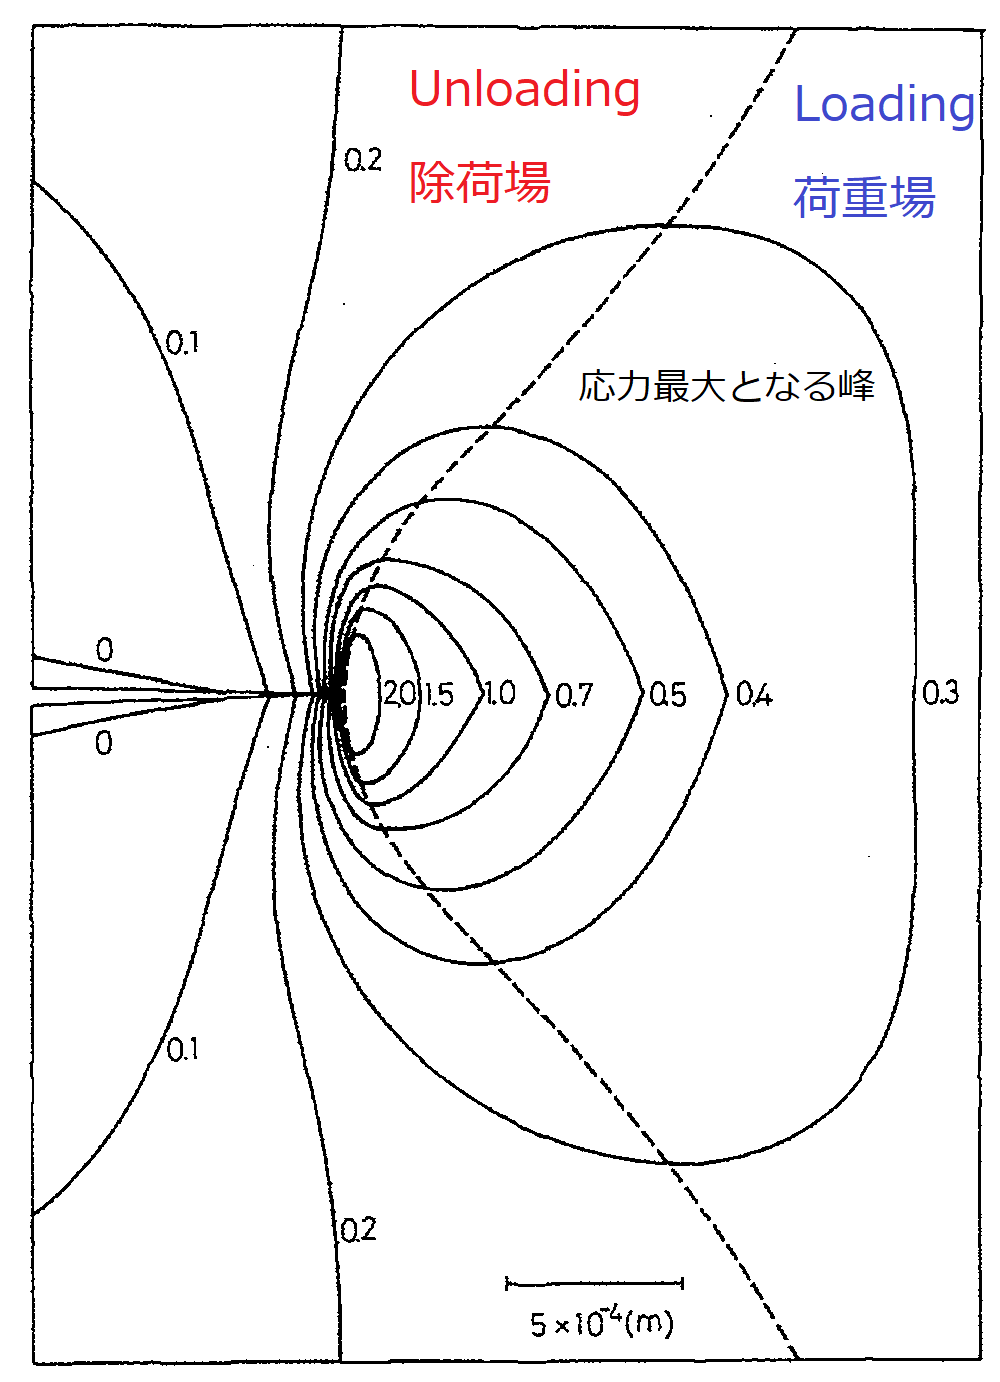
\includegraphics[width=\textwidth]{./crack.png}
	\end{columns}
	
	\begin{alertblock}{クラック先端での力学的ヒステリシス}
	ミクロな緩和現象がマクロな耐久性向上と繋がる。
	\end{alertblock}
\end{frame}

\subsection{ランダムな接続性を有するネットワーク}
% \begin{frame}
% 	\frametitle{ゴムの強靭性}
%     \begin{block}{ヒステリシスについてのこれまでの検討}
%             \begin{itemize}
%                 \item フィラーの添加効果\footnote{
%                     \scriptsize{K. A. Grosch et al., Rub. Chem. and Tech.41, 1157 (1968)}
%                 }

%                 一般に、Mullins 効果と呼ばれるフィラー添加時のヒステリシスと、破断エネルギーとの関係を議論

%                 \item フィラー近傍でのナノキャビティーの開閉\footnote{
%                     \scriptsize{H. Zhang et al., Macromolecules 46, 900 (2013)}
%                 }

%                 フィラー添加時のヒステリシスの起源として、フィラー近傍でのナノキャビティーを議論
%             \end{itemize}
%     \end{block}
%     % \end{columns}
%     \begin{alertblock}{疲労破壊も考慮すると}
%         \begin{itemize}
%             \item \alert{可逆的}であることが望ましい。\textcolor{blue}{$\neq$ 犠牲結合}
%             \item 変形の周期に対応できるように、\alert{回復速度}も重要。
%         \end{itemize}
%     \end{alertblock}
% \end{frame}

% \begin{frame}
%     \frametitle{古典ゴム弾性理論}
%         \vspace{-6mm}
%         \begin{columns}[T, onlytextwidth]
%             \column{.48\linewidth}
%                 \begin{block}{ひずみ不変量に対して}
%                     \begin{itemize}
%                         \item 自由エネルギー密度変化の一般式
%                         \vspace{-3mm}
%                         \scriptsize
%                         \begin{align*}
%                             \dfrac{F}{V} &= \sum_{i,j = 0}^{\infty} C_{ij}(I_1-3)^i(I_2-3)^j \\
%                             &= C_0 + C_1 (I_1-3) + C_2(I_2-3) \\
%                             &\;\;\;\;\;+ \sum_{i,j = 1}^{\infty} C_{ij}(I_1-3)^i(I_2-3)^j
%                         \end{align*}
%                         \normalsize
%                         \item Mooney-Rivlin の式
%                         \vspace{-3mm}
%                         \scriptsize
%                         \begin{align*}
%                             \dfrac{F}{V} &= C_1 (I_1-3) + C_2(I_2-3)
%                         \end{align*}
%                         \normalsize
%                         \item Neo-Hookean 固体
%                         \vspace{-3mm}
%                         \scriptsize
%                         \begin{align*}
%                             \dfrac{F}{V} &= C_1 (I_1-3)
%                         \end{align*}
%                         \normalsize
%                     \end{itemize}
%                 \end{block}
%             \column{.48\linewidth}
%                 \begin{exampleblock}{ミクロな変形モデル}
%                     Neo-Hookean 固体の\\一軸伸張では、
%                     \begin{itemize}
%                         \item Affine Network Model
%                             \begin{itemize}
%                                 \item アフィン変形を仮定
%                             \end{itemize}
%                             \vspace{-3mm}
%                             \scriptsize
%                             \begin{align*}
%                                 \sigma_{nom} &= \textcolor{red}{\nu} k_B T \left(\lambda - \dfrac{1}{\lambda^2}\right) \\
%                                 &= G_{affine} \left(\lambda - \dfrac{1}{\lambda^2}\right)
%                             \end{align*}
%                             \normalsize
%                         \item Phantom Network Model
%                         \vspace{-5mm}
%                             \begin{itemize}
%                                 \item \alert{架橋点ゆらぎ}を考慮
%                                 \item 架橋点の分岐数 $f$
%                             \end{itemize}
%                             \vspace{-3mm}
%                             \scriptsize
%                             \begin{align*}
%                                 G_{phantom} &= \nu k_B T \left(1 - \dfrac{2}{f}\right) \\
%                             \end{align*}
%                             \normalsize
%                     \end{itemize}
%                 \end{exampleblock}
%         \end{columns}       
% \end{frame}

\begin{frame}
	\frametitle{架橋点近傍の拘束状態に基づく二つのモデル}
		\begin{columns}[totalwidth=1\textwidth]
			\column{.45\textwidth}
				\begin{block}{ストランドと架橋点}
					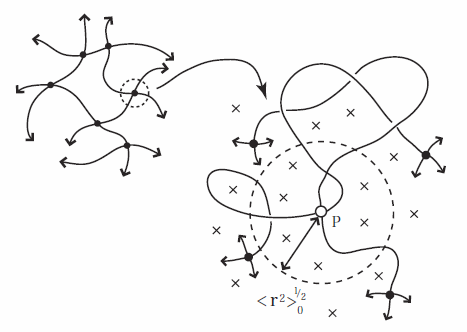
\includegraphics[width=\textwidth]{JP_vicinity.png}
					架橋点はストランド経由で直接連結した架橋点以外の、
					\alert{近接する多数のストランド(図中の×)に囲まれている。}
				\end{block}
			\column{.52\textwidth}
			\begin{itemize}
				\item ``Affine NW Model''\\
					架橋点は周辺に強く拘束され巨視的変形と相似に移動。(Affine 変形)
					\footnotesize
					\begin{align*}
						&G=\nu k_B T \\
						&\text{$\nu$ は、ストランドの数密度}
					\end{align*}
					\normalsize
				\item ``Phantom NW Model''\\
					架橋点が大きく揺らぎ、ずり弾性率($G$)が低下。
					\footnotesize
					\begin{align*}
						&G=\xi \nu k_B T \\
						&\xi= 1 -\dfrac{2}{f}\\
						&\text{$f$ は架橋点の分岐数}
					\end{align*}
			\end{itemize}
		\end{columns}
\end{frame}


\begin{frame}
    \frametitle{ランダムな接続性の導入}
    \vspace{-3mm}
		\begin{columns}[totalwidth=1\textwidth]
			\column{.45\textwidth}
				\begin{block}{接続のランダム性を導入}
					\begin{itemize}
						\item 接続性を不均一に
							\begin{itemize}
								\item 接続に\alert{位置依存性}
							\end{itemize}
						\item 巨視的な変形後
							\begin{itemize}
								\item 結節点のゆらぎが\\不均一
								\item 多様な緩和モード
								\item \alert{緩和の長時間化?}
							% \item ファントムネットワークモデルの諸特性の発現?
							\end{itemize}
						\item \alert{解析を容易}に、
                            \begin{itemize}
                                \item 既往研究で反応系
								\item ストランド長と\\結合数を一定
							\end{itemize}
					\end{itemize}
				\end{block}
			\column{.52\textwidth}
				ランダム構造の模式図
				\vspace{5mm}
				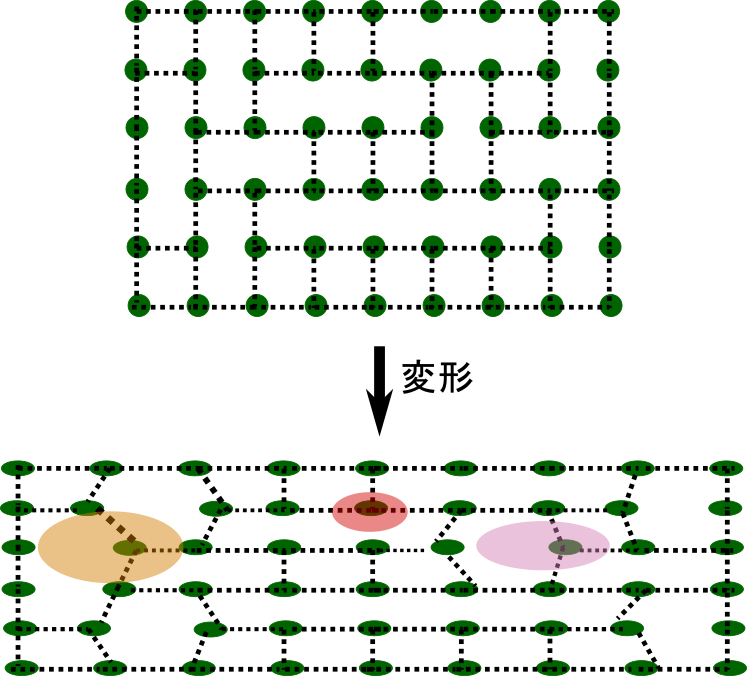
\includegraphics[width=\textwidth]{random_NW.png}
    \end{columns}
\end{frame}


\begin{frame}
	\frametitle{本発表の内容}
		\begin{exampleblock}{ランダムな接続性を有するネットワークポリマー}
			\begin{itemize}
				\item ネットワーク構造の接続性にランダム性を導入
				\begin{itemize}
					\item 各ノードごとにランダムな結合性を導入
					\item ストランドの末端間距離がガウス分布
					% する\\ランダムネットワーク構造
				\end{itemize}
			\item ランダムネットワーク構造の力学的応答
				\begin{itemize}
					\item 応力緩和関数
					\item 一軸伸長での変形速度依存性
				\end{itemize}
				\item 絡み合いの影響を確認
				\begin{itemize}
					\item PPA での絡み合いの可視化
					\item Z1-code による比較
				\end{itemize}
				\item ヒステリシスの確認
				% \begin{itemize}
				% 	\item PPA での絡み合いの可視化
				% 	\item Z1-code による比較
				% \end{itemize}
			\end{itemize}
		\end{exampleblock}
\end{frame}

\section{KG鎖でのシミュレーション結果}

\subsection{ランダムな接続性を有するネットワークポリマー}
\begin{frame}
	\frametitle{ランダムな接続性を有するネットワーク}
	\vspace{-1mm}
		\begin{exampleblock}{作成のアルゴリズム}
			\begin{enumerate}
				\item \alert{実空間}で8-Chain Model で初期構造を作成。
					\begin{itemize}
						% \item \alert{実空間}で8-Chain Model で初期構造を作成。
						% \item 所望の分岐数に\alert{ランダム}に選択した\alert{結合を除去}
						\item 除去したジオメトリーに対応した\alert{トポロジーモデル}
					\end{itemize}
				\item トポロジー空間でランダム性の導入
					\begin{itemize}
						% \item ラプラシアン行列で全体の接続性を確認しながら、
						\item \alert{エッジ交換}して、ネットワーク構造にランダムな接続性を導入
					\end{itemize}	
				\item 対応する\alert{実空間でのネットワーク初期構造}を作成
				\item ストランド長がホモポリマーに対応するように多重度設定して、Slow Push Off により初期構造を緩和
			\end{enumerate}
		\end{exampleblock}
		\vspace{-1mm}
		\begin{columns}[T, onlytextwidth]
			\column{.33\linewidth}
				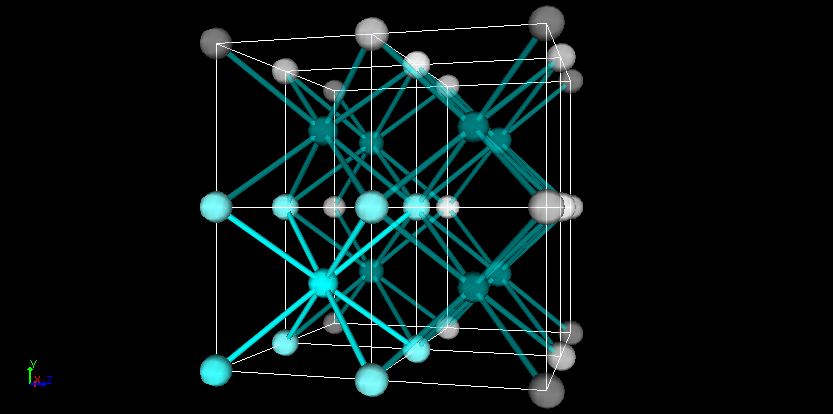
\includegraphics[width=\textwidth]{8_per.png}
			\column{.33\linewidth}
				\vspace{-5mm}
				\begin{center}
					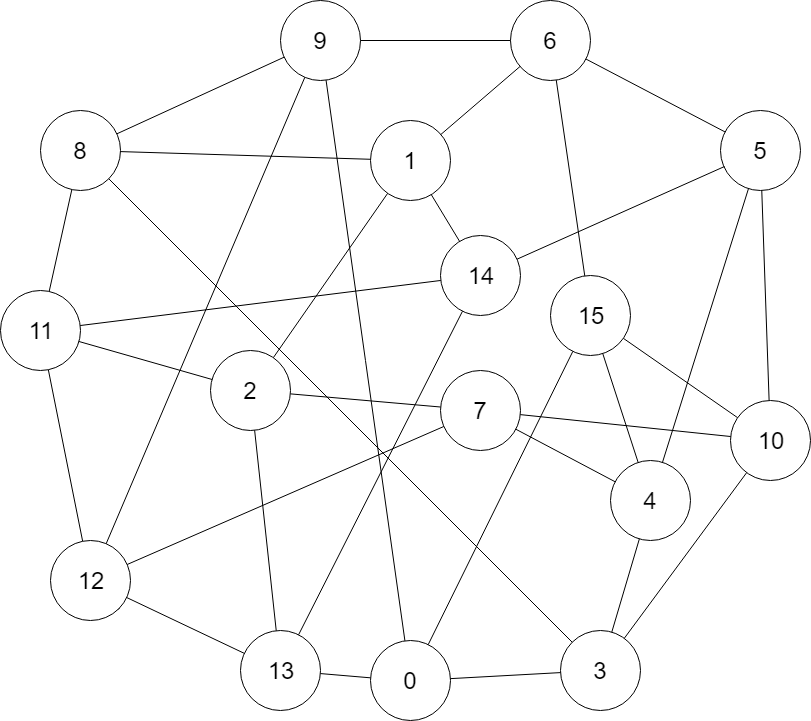
\includegraphics[width=.6\textwidth]{Network.png}
				\end{center}
			\column{.33\linewidth}
				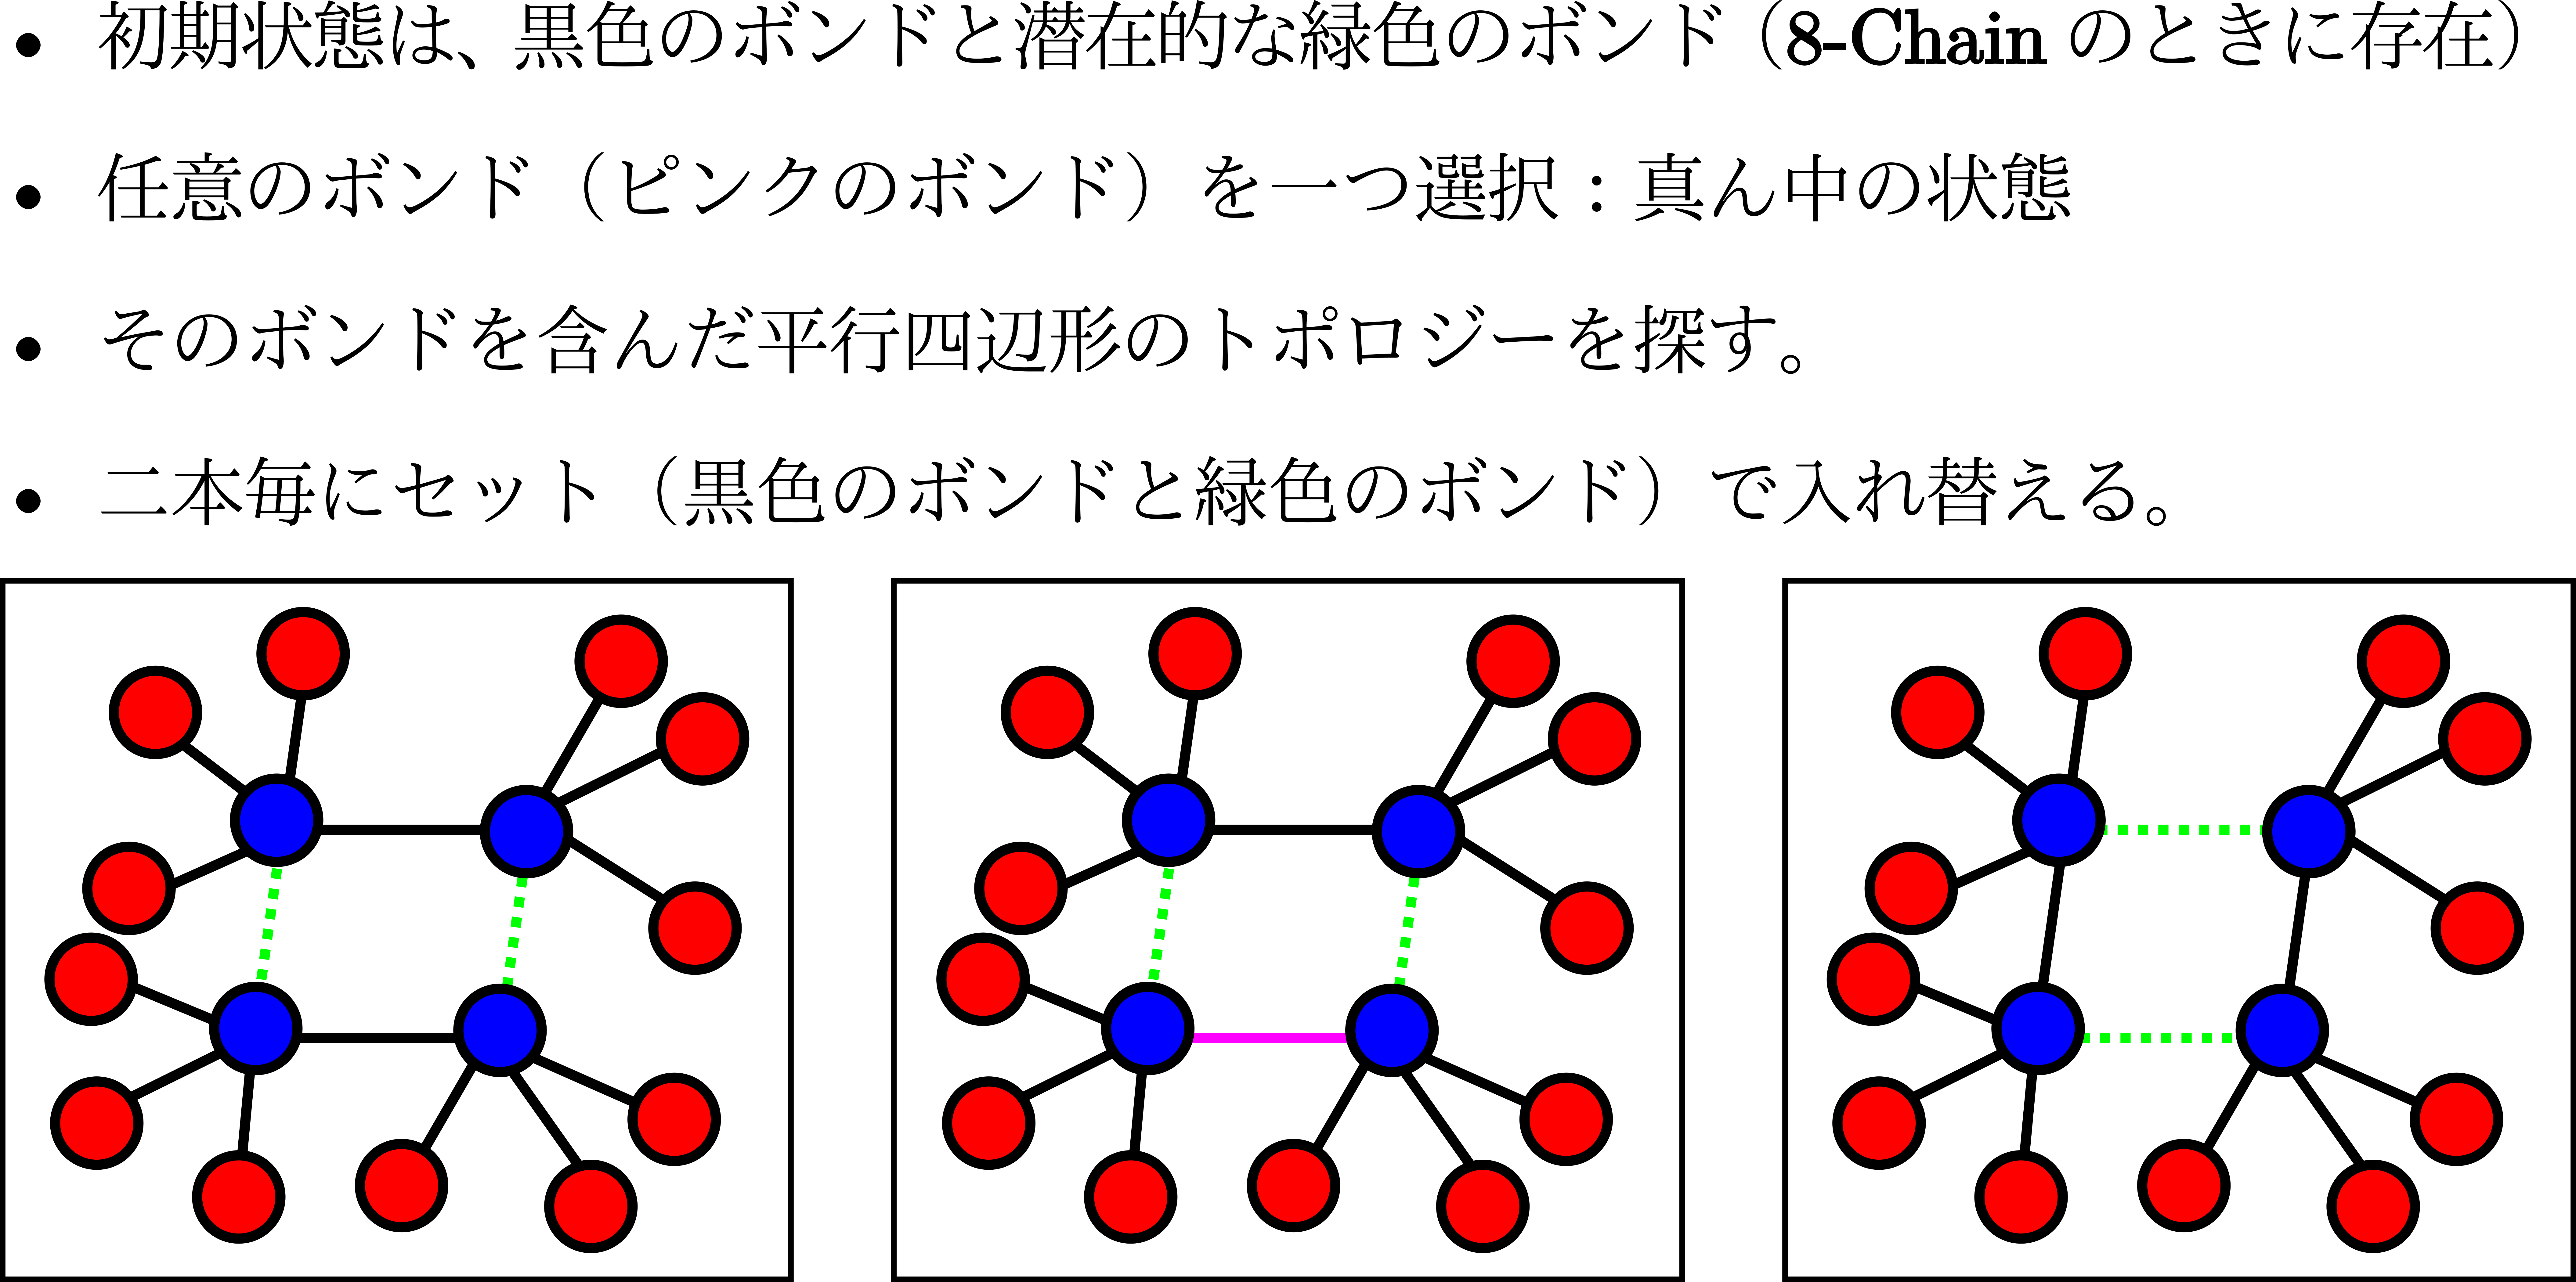
\includegraphics[width=\textwidth]{bond_exchg.png}
		\end{columns}
\end{frame}

\subsection{力学的な応答}
\begin{frame}
	\frametitle{四分岐ネットワークの力学応答}
		\begin{columns}[T, onlytextwidth]
			\column{.48\linewidth}
				\begin{block}{一軸伸張結果}
					\begin{itemize}
						\item 伸張速度の低下によりネオフッキアンに漸近
						\item ANMよりも応力は高い
					\end{itemize}
					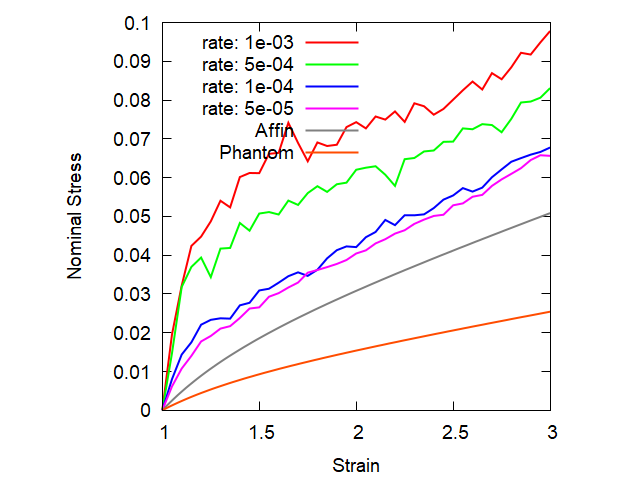
\includegraphics[width=\textwidth]{N48_C4_M3.png}
				\end{block}
				
			\column{.48\linewidth}
				\begin{block}{応力緩和関数 $G(t)$}
					\begin{itemize}
						\item ステップ変形($\lambda=2.0$)
						\item 最長緩和の長時間化
						\item ANM よりも高弾性率
					\end{itemize}
					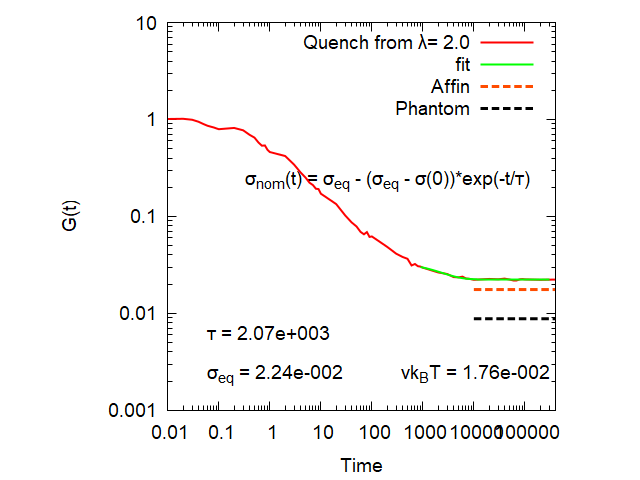
\includegraphics[width=\textwidth]{gt_N48_C4_M3.png}
				\end{block}
		\end{columns}
\end{frame}

\begin{frame}
    \frametitle{Z1-code での確認}
        \vspace{-3mm}
        \begin{columns}[T, onlytextwidth]
            \column{.4\linewidth}
                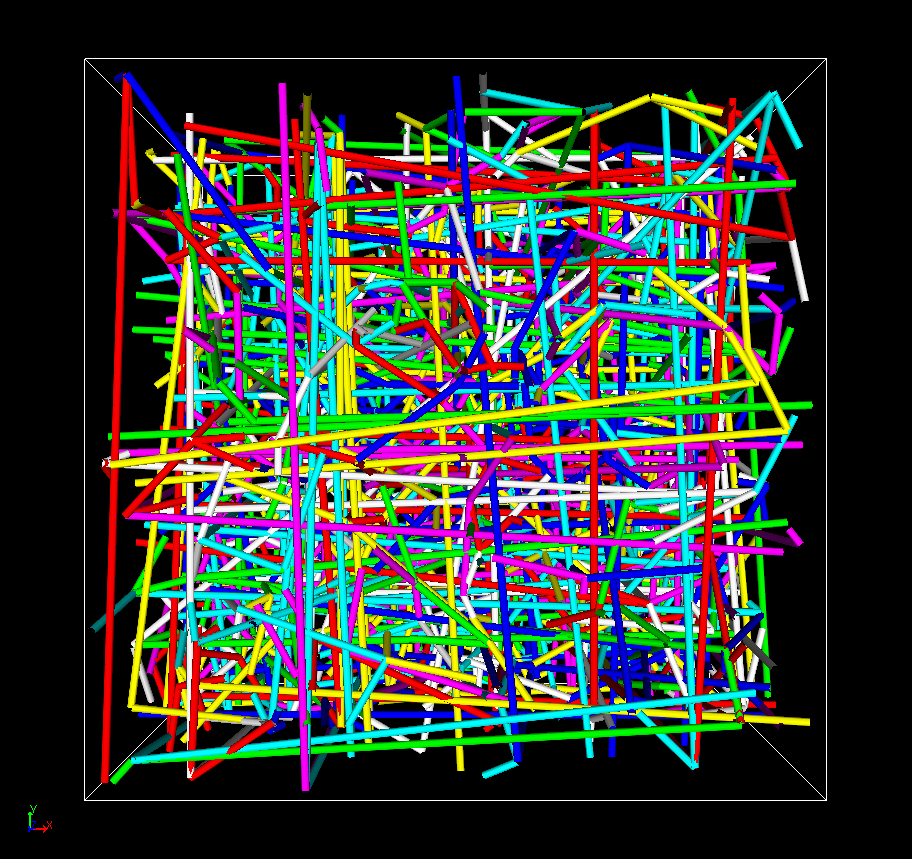
\includegraphics[width=\textwidth]{z_cord_4Chain.png}
                Z1-code での絡み合い
            \column{.56\linewidth}
            \begin{block}{ホモポリマーとの比較}
                \begin{itemize}
                    \item Z は一本鎖あたりの絡み合い
                    \item 今回のネットワークは、\\ホモポリマーと同等
                \end{itemize}
                \scriptsize
                \begin{center}
                    \begin{tabular}{c||c|c} \hline
                        &Homo & 4 Chain NW \\ \hline \hline
                        Segments& 50& 48 \\ \hline
                        Chains & 200& 768 \\ \hline
                        Entanglements& 204& 800\\ \hline
                        Entangled Chains&134&557 \\ \hline
                        \alert{$<Z>_{Z1}$}&\alert{1.02}& \alert{1.04}\\ \hline
                    \end{tabular}
                \end{center}
            \end{block}
        \end{columns}
    \begin{alertblock}{Z1-codeとは}
        \begin{itemize}
            \item 絡み合いを可視化するアルゴリズム\footnote{
                M. Kröger, Comput. Phys. Commun. 168, 209 (2005)
                % \begin{itemize}
                %     \item M. Kröger, Comput. Phys. Commun. 168, 209 (2005)
                %     \item S. Shanbhag, M. Kröger, Macromolecules 40, 2897(2007)
                %     \item R. Hoy, K. Foteinopoulou, M. Kröger, Phys. Rev. E, 31803 (2009)
                % \end{itemize}
            }
        %    N.C. Karayiannis, M. Kröger, Int. J. Mol. Sci. 10, 5054 (2009)
        \end{itemize}
    \end{alertblock}
\end{frame}

\subsection{絡み合いを低減したネットワーク}
\begin{frame}
	\frametitle{絡み合いを低減したネットワーク}
		\begin{exampleblock}{NPT 計算での初期構造の緩和}
			\begin{itemize}
				\item \alert{密度の低い初期状態}から NPT 計算により圧縮して、
				\item 絡み合いを極力排除した初期構造を作成した。
			\end{itemize}
		\end{exampleblock}

		\begin{columns}[T, onlytextwidth]
			\column{.48\linewidth}
				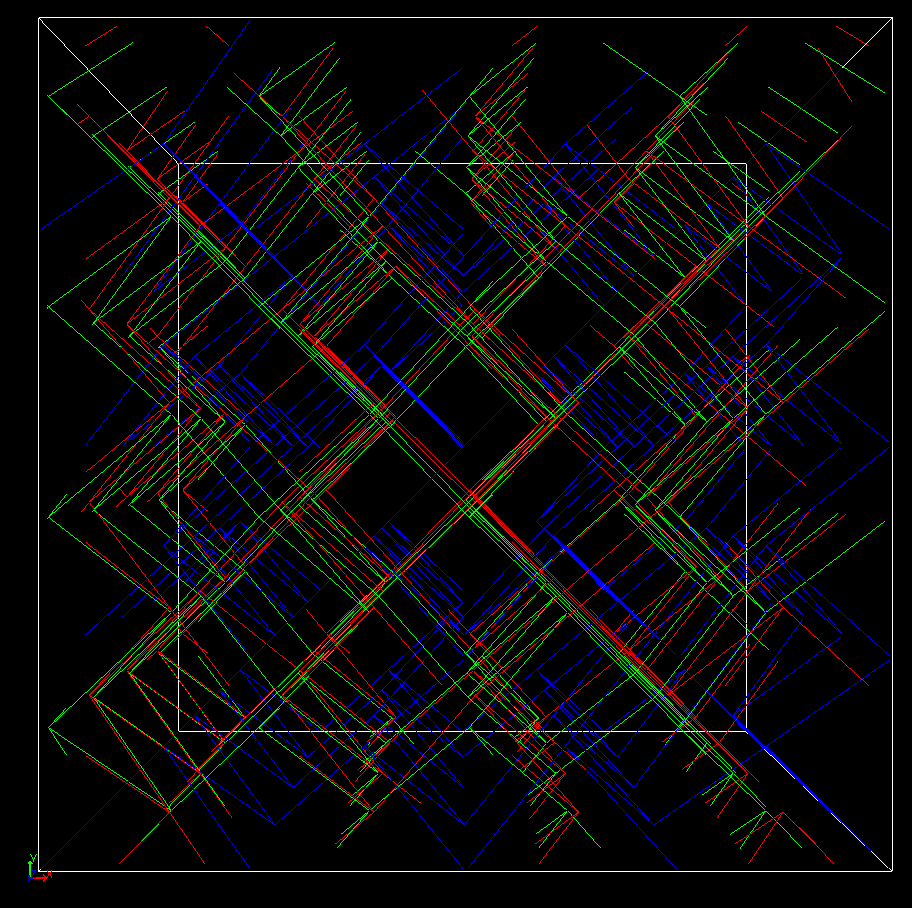
\includegraphics[width=.9\textwidth]{NPT_00.png}
			\column{.48\linewidth}
				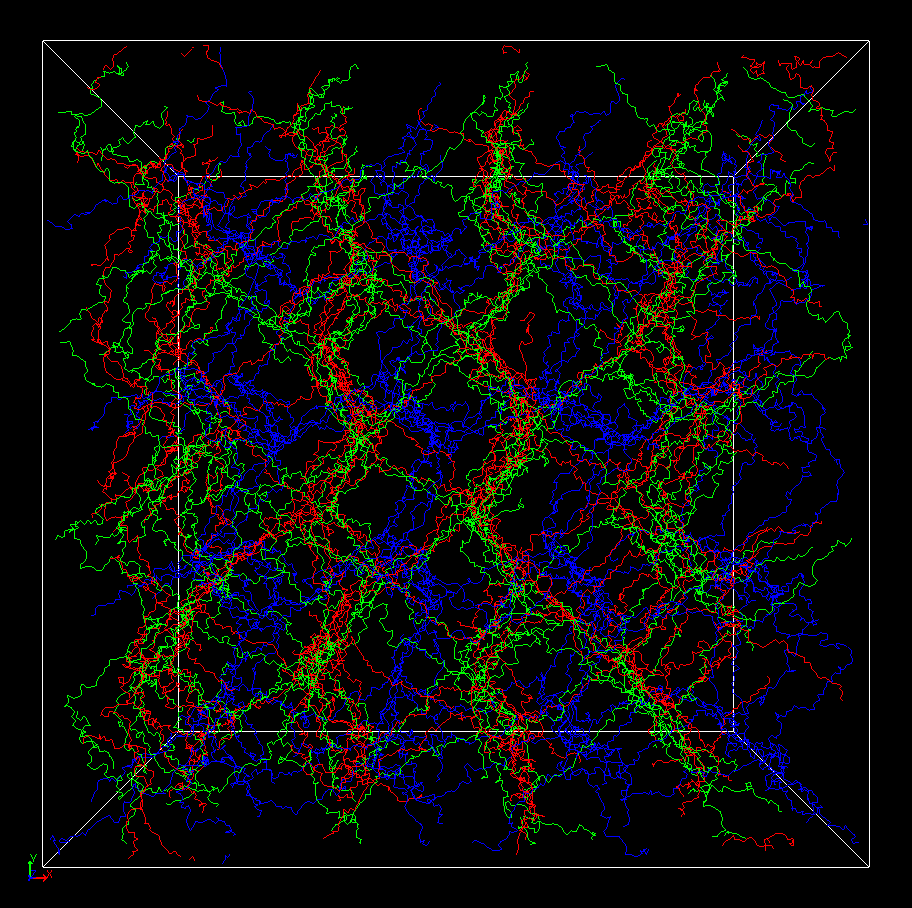
\includegraphics[width=.9\textwidth]{NPT_11.png}
		\end{columns}
\end{frame}

\begin{frame}
    \frametitle{絡み合いを低減したネットワーク}
        \vspace{-3mm}
		\begin{columns}[T, onlytextwidth]
            \column{.4\linewidth}
			\begin{exampleblock}{PPAでの絡み合い}
				\small
				\begin{itemize}
					\item 4-Chain-\alert{NPT}
					
					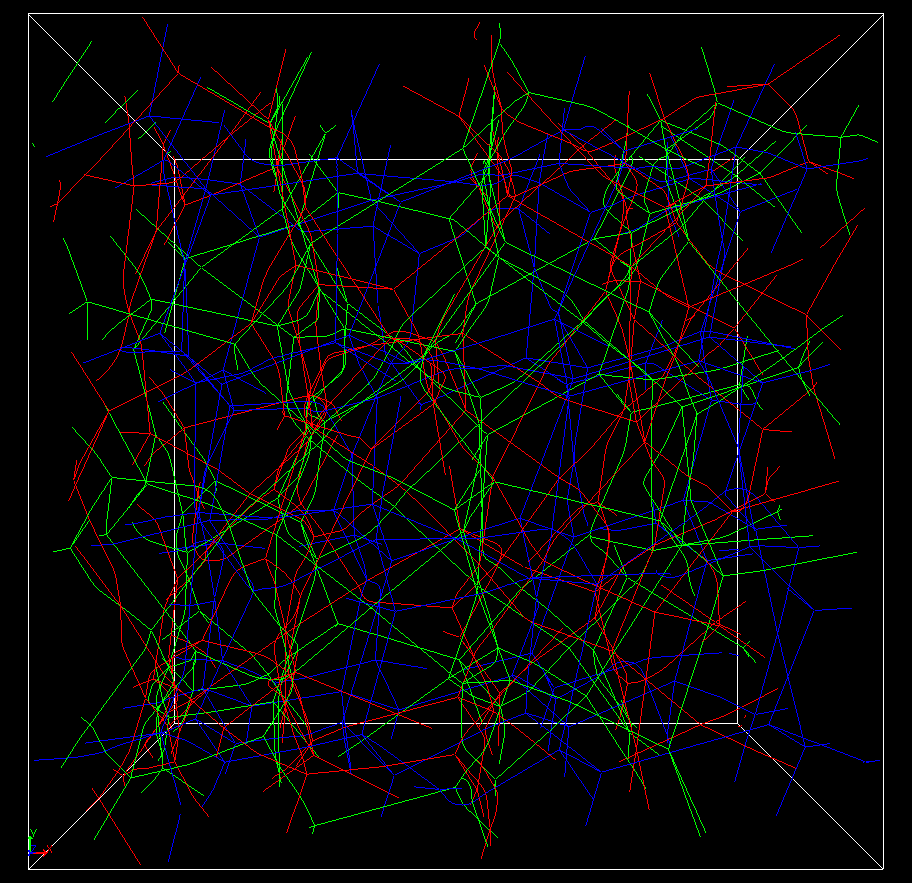
\includegraphics[width=.58\textwidth]{NPT_PPA.png}
					\item 4-Chain-NVT
					
					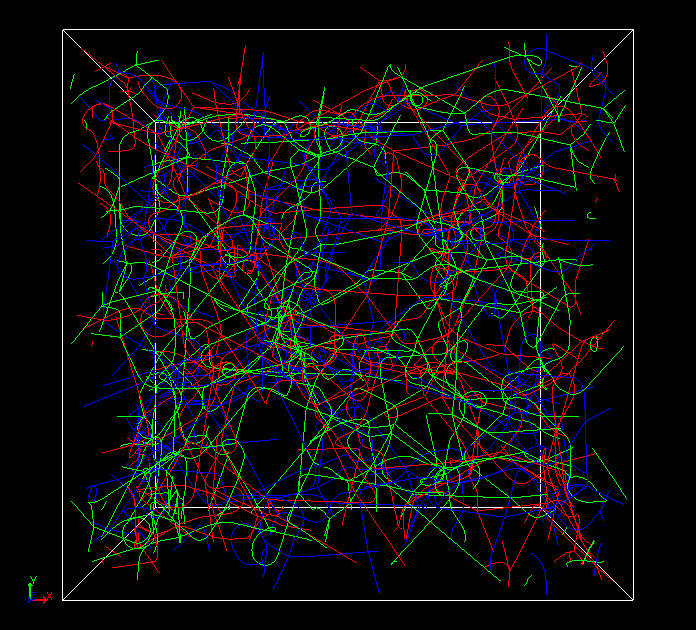
\includegraphics[width=.58\textwidth]{N48_f4_PPA.png}
				\end{itemize}
			\end{exampleblock}
                
			\column{.56\linewidth}
			\begin{block}{応力緩和関数 $G(t)$}
				\begin{itemize}
					\item ステップ変形($\lambda=2.0$)
					\item 弾性率がPNMに漸近
					% \item<2> \textcolor{blue}{定数を足せばKGと類似}
				\end{itemize}
				\vspace{6mm}
					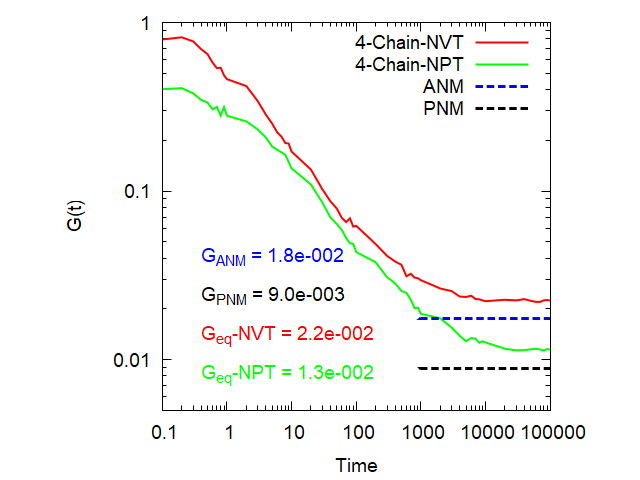
\includegraphics[width=\textwidth]{gt_4chain_comp.png}
					% \includegraphics<2>[width=\textwidth]{gt_NPT_mod.png}
				\end{block}
		\end{columns}
\end{frame}

\begin{frame}
    \frametitle{絡み合いの効果について}
	\footnotesize
		M. Rubinstein, S. Panyukov, Macromolecules, 35, 6670 (2002)
			\begin{align*}
				&G_c = \nu k_B T \left(1-\dfrac{2}{\phi} \right), \quad G_e = \dfrac{4}{7} \nu k_B T L \\
				&\text{where $\nu$ is the number density of network chains,} \\
				& \text{and L is the number of slip-links per network chain}
			\end{align*}
		\vspace{-10mm}
		\begin{columns}[c, onlytextwidth]
			\column{.3\linewidth}
				\vspace{-3mm}
				\begin{center}
					% 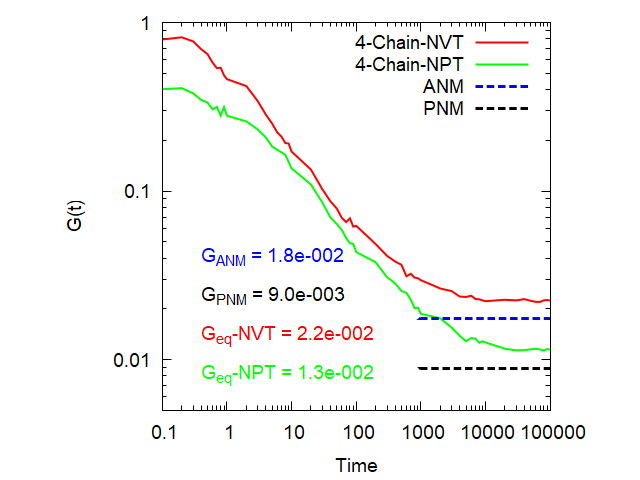
\includegraphics[width=\textwidth]{gt_4chain_comp.png}
					
					% \vspace{3mm}
					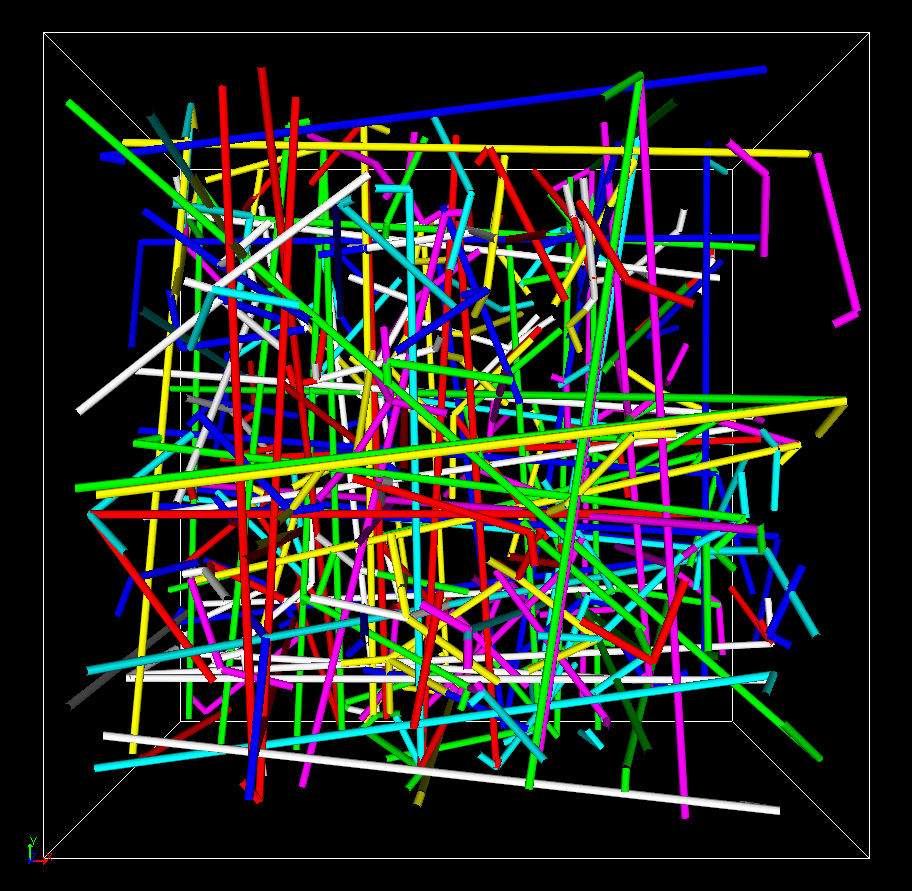
\includegraphics[width=.9\textwidth]{z_cord_NPT_4Chain.png}

					\scriptsize
					Z1-code for NPT
				\end{center}
			\column{.65\linewidth}
				\scriptsize
				\begin{center}
					\begin{tabular}{c|c|c} \hline
						&NPT & NVT \\ \hline \hline
						\textcolor{blue}{Chains} & \multicolumn{2}{|c}{\textcolor{blue}{768}}\\ \hline
						\textcolor{blue}{$\nu$}& \multicolumn{2}{|c}{\textcolor{blue}{0.018}}\\ \hline
						\textcolor{blue}{$G_c = \nu \times (1-2/4)$}&\multicolumn{2}{|c}{\textcolor{blue}{0.009}} \\ \hline \hline
						Entanglements& 278& 800\\ \hline
						Entangled Chains&249&557 \\ \hline
						L & 278/768=0.36 & 800/768=1.04 \\ \hline
						$G_e=4/7 \times \nu \times L $ & 0.004 & 0.011 \\ \hline \hline
						$G_{calcd.}=G_c + G_e$ & 0.013 & 0.020 \\ \hline \hline
						$G_{measd.}$ & 0.013 & 0.022 \\ \hline
					\end{tabular}
				\end{center}
		\end{columns}
\end{frame}

\begin{frame}
    \frametitle{ヒステリシスの検討}
        \begin{block}{計算条件}
            \begin{itemize}
                \item 変形:一軸伸長、コーシーひずみ
                \item 伸張速度:$\dot{\lambda} = 1E-4 [1/\tau]$
            \end{itemize}
        \end{block}
    \begin{columns}[T, onlytextwidth]
        \column{.48\linewidth}
        \begin{itemize}
            \item 4-Chain-NVT
        \end{itemize}
            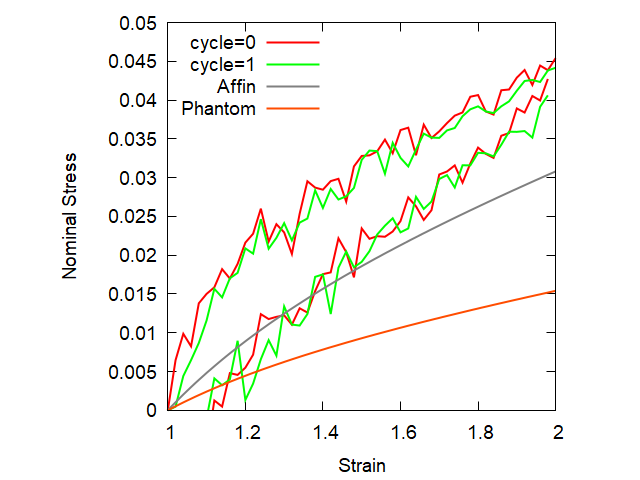
\includegraphics[width= \textwidth]{hyst_4Chain.png}
        \column{.48\linewidth}
        \begin{itemize}
            \item 4-Chain-NPT
        \end{itemize}
            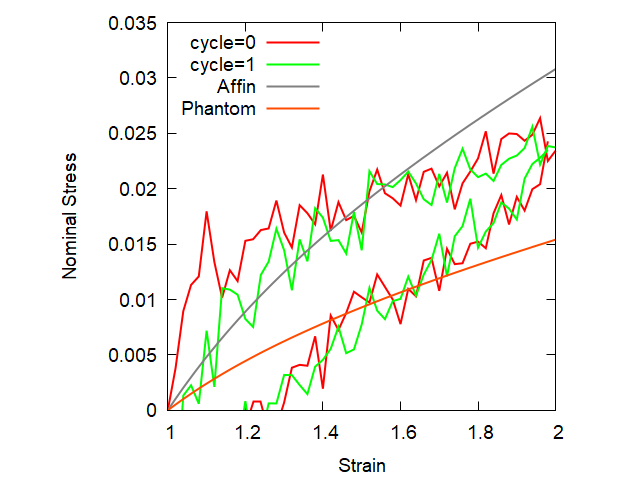
\includegraphics[width=\textwidth]{hyst_NPT_4Chain.png}
    \end{columns}
\end{frame}

\begin{frame}
    \frametitle{緩和状態の比較}
	\begin{exampleblock}{動的粘弾性スペクトルの作成}
		\begin{itemize}
			\item 平衡状態での応力ゆらぎの相関関数を測定
			\item Green-Kubo により、応力緩和関数G(t) を得る。
			\item 必要に応じて、長時間側を外挿。
			\item 離散データを線形近似で内挿し動的粘弾性スペクトル
		\end{itemize}
	\end{exampleblock}
    \begin{columns}[onlytextwidth]
        \column{.5\linewidth}
            \begin{itemize}
                \item ネットワークをホモポリマーと比較
                \begin{itemize}
                    \item 絡み合いを抑制した NPT はホモポリマーに類似
                    \item NVT では、ストランドの自由な運動が抑制?
                \end{itemize}
                % \item \textcolor{red}{3分岐のほうが、長時間緩和を持っていた。}
            \end{itemize}
        \column{.48\linewidth}
            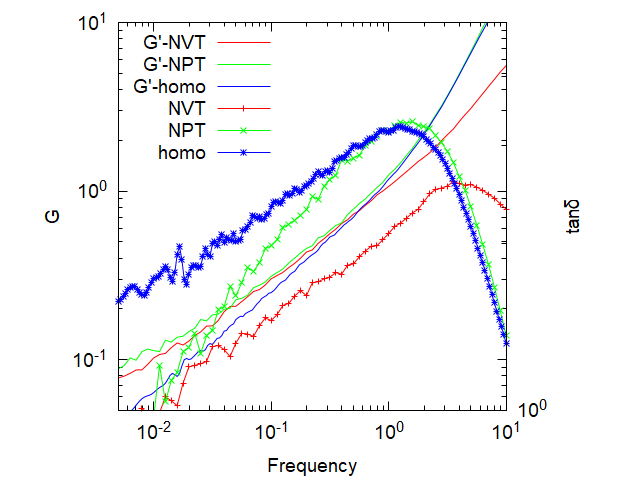
\includegraphics[width=\textwidth]{gw_eq.png}
    \end{columns}
\end{frame}

\begin{frame}
	\frametitle{おわりに}
		\begin{block}{本発表の内容}
			\begin{itemize}
			\item ネットワーク構造の接続性にランダム性を導入
				\begin{itemize}
					\item 各ノードごとにランダムな結合性を導入
					\item ストランドの末端間距離がホモポリマーと対応するランダムなネットワーク構造
				\end{itemize}
			\item ランダムネットワーク構造の力学的応答
				\begin{itemize}
					\item 比較的長時間での緩和を確認
					\item アフィンネットワークモデル程度の高い弾性率
				\end{itemize}
			\item 絡み合いを低減したネットワーク構造との比較で、
				\begin{itemize}
					\item 比較的長時間での緩和を確認
					\item Trapped Entanglements が緩和後の弾性率に影響 
					\item ファントムネットワークモデルへと漸近
					\item ヒステリシスの発現が増加
				\end{itemize}
			\end{itemize}
		\end{block}
\end{frame}

\end{document}
